\documentclass[12pt,scrartcl,titlepage]{article}
\renewcommand{\baselinestretch}{1.5}
\usepackage[utf8]{inputenc}
\usepackage[margin=1.15in]{geometry}
\usepackage{setspace}
\usepackage{ifpdf}
\usepackage{amsmath}
\usepackage{amssymb}
\usepackage{fancyhdr}
\usepackage{float}
\usepackage{xcolor}
\usepackage{listings}
\usepackage{graphicx}
\usepackage[parfill]{parskip}
\usepackage{hyperref}
\usepackage{subfig}
\usepackage{mwe}
\usepackage[font=it]{caption}

\pagestyle{fancy}

\newcommand{\HRule}{\rule{\linewidth}{0.5mm}}

\fancyhf{}

\begin{document}

\lhead{G121 Final Project Report}
\rhead{J. Blake, M. Haney, R. Lawson, M. Notaros}
\cfoot{\thepage}

{\setstretch{1.0} \begin{titlepage}
\begin{center}

% Upper part of the page. The '~' is needed because \\
% only works if a paragraph has started.

\textsc{\Large UNIVERSITY OF COLORADO BOULDER}\\[1.5cm]

\textsc{\large ECEN 2270: ELECTRONICS DESIGN LAB FINAL REPORT}\\[0.5cm]

% Title
\HRule \\[0.4cm]
{ \LARGE \bfseries Movement Controlled Robot \\ [0.4cm] }

\HRule \\[1.5cm]

% Author and supervisor
\noindent
\begin{minipage}{0.4\textwidth}
\begin{flushleft} \large
Joseph \textsc{Blake}\\
Matthew \textsc{Haney}
\end{flushleft}
\end{minipage}%
\begin{minipage}{0.4\textwidth}
\begin{flushright} \large
Rachel \textsc{Lawson}\\
Milica \textsc{Notaros}
\end{flushright}
\end{minipage}\\[1.5cm]

\vfill

% Bottom of the page
{\large \today}

\end{center}

\end{titlepage}
 }

\tableofcontents

\pagebreak

% The report should focus on the Lab 6 add-on project components, and how the components are incorporated with the circuits completed in Labs 1-5. Provide a full description of the robot additional control circuits with design, simulation, and experimental results. Describe how the project design is split into more manageable sub-circuits or blocks for design, testing and de-bugging. Comment on design, hardware and code challenges that you had to work through to get the project circuitry fully operational. Propose future extensions to improve the performance and capabilities.

\section{Introduction and Objectives}

For our group's final project we added an additional custom component to our robot that incorporated both hardware and software. Our project consisted of a glove that controls  the direction the robot moves, and a muscle sensor that controls the speed of the robot. The glove has two flex sensors and an accelerometer which combined will drive the robot forward, backwards, left, and right. We also have a muscle sensor that controls the speed by sensing the magnitude of the electrical activity of the muscle. There are three ranges of speeds: fast, medium, and slow. These components communicate wirelessly over WiFi. Overall, This project can be loosely divided into three parts: an array of inputs, a wireless transmitter that encodes the input data into a command, and a wireless receiver that translates the command into an action taken by the robot.

\section{Equipment}
{ \setstretch{1.0}
\noindent Hardware:
  \begin{itemize}
  \item EMG Sensor (Sparkfun Muscle Sensor v3)
  \item Arduino UNO R3
  \item 2x Flex Sensor (FS7548)
  \item Accelerometer (ADXL337)
  \item Teensy 3.1 (PJRC)
  \item TeensyLC (PJRC)
  \item 2x Wireless Transceiver (ESP8266)
  \item Gardening Glove, Duct Tape
  \item Slide Potentiometer
  \item Push Button
  \item AA Batteries
  \item Robot with lab 1-4 components
  \item Agilent DSO1024A Oscilloscope
  \item Agilent E3631A Triple Output DC Power Supply
  \end{itemize}
  
\noindent Software:
  \begin{itemize}
  \item Arduino IDE
  \item PJRC Teensy Software (Arduino IDE Extension) [1]
  \item IntuiLink Data Capture
  \end{itemize}
}
  \section{Methods and Results}

  \subsection{Control Input Design and Testing}

  \subsubsection{Glove Controller Design}

  First we worked on the glove controller, which the user will use to control the movement of the robot. The glove is made up of two flex sensors, an accelerometer, a muscle sensor, a push button, and a slide potentiometer. The flex sensors are attached to the index and middle fingers of the glove. The user chooses the forward or backward direction based on which finger is bent. To make the robot go forward, the user bends their index finger and to make the robot go backward, the user bends their middle finger. The accelerometer chooses the turning direction of the robot. If the user tilts their hand to the left, the robot turns left, and if the user tilts their hand right, the robot turns right. The layout of the glove with the two tilt sensors and accelerometer is shown below.

  \begin{figure}[h!]
    \centering
    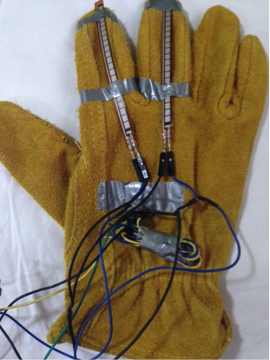
\includegraphics[width=0.3\textwidth]{glove.png}
    \caption{Glove with tilt sensors and accelerometer}
  \end{figure}

  In addition to the sensors shown in Figure 1, the user wears an EMG muscle sensor which detects the level of muscle activity. The user controls the speed of the robot with this sensor. The more the user flexes their muscle, the faster the robot goes. Hence, the direction is chosen with the sensors pictured in Figure 1, and the speed is chosen using the muscle sensor. The muscle sensor is connected to the user via electrode sensor pads. The proper hookup of these pads is shown in Figure 2 below.

  \begin{figure}[h!]
    \centering
    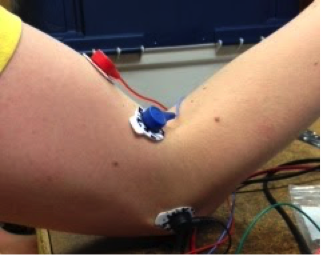
\includegraphics[width=0.3\textwidth]{arm.png}
    \caption{Proper connection of the electrode sensor pads to the muscle}
  \end{figure}

  As can be seen in Figure 2 above, the electrode pads should be connected with the red connector on the middle of the muscle, the blue connector on the bottom of the muscle, and the black connector on a bone near the muscle. Proper connection of the sensor pads is very important to get a clear signal from the sensor. The muscle sensor provides a very interactive way to control the speed of the sensor. One drawback with EMG control is that the electrode sensor pads are supposed to be used only once and then thrown away, so it is not very feasible to pass the muscle controls between users. Due to this fact, we designed a second control mode which uses a different type of speed control. The user can enter the second mode by pressing a push button. In the second mode, the user still uses the glove pictured in Figure 1 to choose the direction of the robot, as the glove is easy to switch between multiple users, but the speed is then chosen via the slide potentiometer. There is also a LCD screen which prints important sensor values and tells the user which mode they are in for convenience.
  
  \subsubsection{Muscle Sensor Testing}

  We tested the EMG muscle sensor to see how well it responds to a user’s muscle activity. We powered the muscle sensor with the power supply and connected the output signal to the oscilloscope, as shown in Figure 3 below.
  
  \begin{figure}[h!]
    \centering
    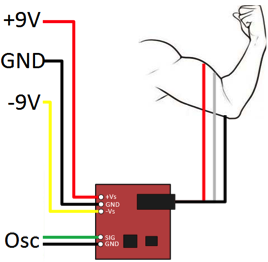
\includegraphics[width=0.3\textwidth]{msv3-setup.png}
    \caption{Muscle sensor testing connections}
  \end{figure}

  We did testing with +-9V, as that is the recommended voltage for the sensor. We found that the sensor responds very well to muscle activity. Plots of the signal output for the resting position, high bursts of muscle activity, and gradual increase in muscle activity are shown below.

\begin{figure}[h!]
  \begin{minipage}{.5\linewidth}
    \centering
    \subfloat[]{\label{main:a}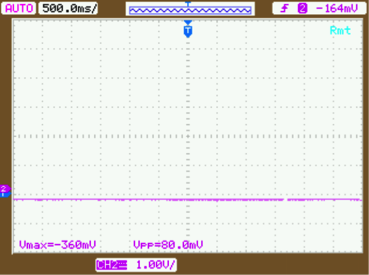
\includegraphics[scale=]{plot-a.png}}
  \end{minipage}%
  \begin{minipage}{.5\linewidth}
    \centering
    \subfloat[]{\label{main:b}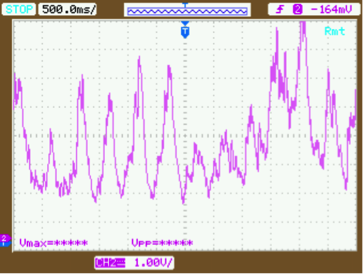
\includegraphics[scale=1]{plot-b}}
  \end{minipage}\par\medskip
  \centering
  \subfloat[]{\label{main:c}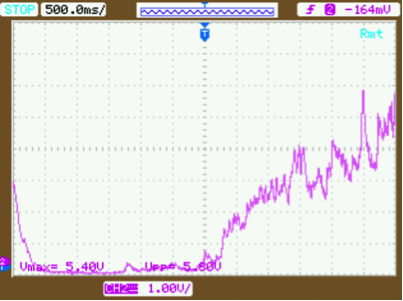
\includegraphics[scale=1]{plot-c}}
  \begin{center}
    \caption{Muscle sensor output signal: (a) no muscle activity/resting; (b) high spikes of movement; (c) gradual increase in muscle activity}
  \end{center}
\end{figure}

  As can be seen in Figure 4 above, the muscle sensor detects muscle activity very well. When the user is resting, the output signal is very steady at a low voltage. When the user makes drastic movements, the output signal has huge spikes in voltage. It is also possible for the user to gradually increase the signal voltage by gradually flexing harder. We were able to get a good range of low, medium, and high amount of muscle activity that the user can easily differentiate between and maintain comfortably.

  Although $\pm$9V is the recommended input voltage, it is too high for the Teensy. We then powered the signal with +3.3V from the Teensy and -5V from a battery pack. Although the positive and negative voltage rails were not equal, the hardware had no problem working correctly. The positive rail was powered by the Teensy so that it did not receive input signals that would damage it. We then connected the output signal of the muscle sensor to an analog pin on the Teensy in order to read the values that the sensor produces. We found that the sensor produces a very steady signal for the different ranges of muscle activity. There is a significant difference in the output value based on the muscle activity of the user. We tested the sensor for various ranges of muscle activity. The results are seen below in Table 1.

  \begin{table}[h!]
    \begin{center}
      \begin{tabular}{|c|c|}
        \hline
        \textbf{Muscle Activity}&\textbf{Sensor Value}\\
        \hline
        Resting&85-95\\
        \hline
        Low&100-150\\
        \hline
        Medium&180-250\\
        \hline
        High&400-1023\\
        \hline
      \end{tabular}
    \end{center}
    \caption{Sensor values for various muscle activity ranges}
  \end{table}

  As shown in Table 1 above, we were able to get good ranges for the different muscle activity levels. They are easy to achieve and maintain by the user. The four ranges shown above correspond to the different robot speeds, where resting is our lowest speed and high is the maximum speed.
  
  \subsubsection{Flex Sensor and Accelerometer Testing}

  The accelerometer has three axes on it; however, we only use one axis, as we only need to be able to detect tilting in one direction. Therefore, we leave two of the axis signal outputs unconnected. We tested the sensor with it connected to the Teensy to see what values are outputted for different tilt ranges.
  \begin{table}[h!]
    \begin{center}
      \begin{tabular}{|c|c|}
        \hline
        \textbf{Tilt}&\textbf{Sensor Value}\\
        \hline
        Left&$V \geq 670$\\
        \hline
        Right&$V \leq 550$\\
        \hline
      \end{tabular}
    \end{center}
    \caption{Sensor values for left and right tilt orientation}
  \end{table}

As seen above in Table 2, when the user tilts the glove left, the value read from the accelerometer is above 670, and when the user tilts the glove right, the value read is below 550. When the sensor is outputting a value between the two values seen in Table 2 it constitutes as the user keeping their hand flat, and therefore the robot does not turn.

The flex sensors were tested in a similar manner. The flex sensor is a variable resistor, and we connected each of them in series with a 22k$\Omega$ resistor, creating a voltage divider, where the upper resistor was the flex sensor. The center node was then connected to an Analog Input pin on the Teensy.

  \begin{figure}[h!]
    \centering
    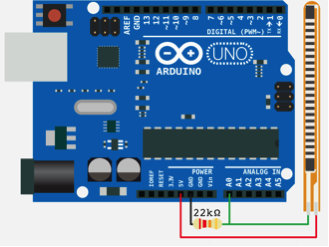
\includegraphics[width=0.3\textwidth]{flex.png}
    \caption{Connection of a flex sensor to an Arduino (in our case a Teensy)}
  \end{figure}

We found cutoff values for when the flex sensor is bent an appropriate amount. The value is 550 for the forward control flex sensor and 600 for the backward control flex sensor. It is interesting to note that the values for the two flex sensors are slightly different. This is most likely due to inherent tolerances within the flex sensors or resistors.

  \subsubsection{Push Button and Potentiometer Implementation}

  As stated earlier, the push button and slide potentiometer are used to implement a second mode during which the user can control the speed of the robot with the potentiometer rather than the EMG muscle sensor. This second mode is entered when the push button is pressed. Then the user can return back to the first mode by pressing the button again. The potentiometer controls the speed from 0\% to 100\% based on what position it is slid to.
  
  \subsection{Wireless Connection and Final Implementation}

  \subsubsection{Wireless Setup and Code}

To communicate wirelessly with the robot, we chose to use a pair of ESP8266 wireless modules, one of which created a WiFi Access Point and ran the TCP server, the other of which connected to the AP. Although commands were only sent to the robot, bi-directional communication is feasible with this chip. A Teensy 3.1 and a Teensy LC were chosen due to having hardware serial with hardware buffers and 3.3V logic like the ESP8266 module, making communication easier than with an Arduino. We already had a Teensy 3.1 for the transmitting end and the LC version was purchased for the receiving end. This configuration led to an implementation using three microcontrollers to translate an array of inputs into outputs, as shown in the block diagram in Figure 7. The connection was handled using bi-directional logic level converters using the MOSFETs provided in our lab kit.

\begin{figure}[h!]
  \centering
  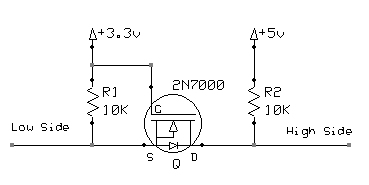
\includegraphics[width=0.5\textwidth]{level-shifter.png}
  \caption{Example bi-directional logic level shifter schematic}
\end{figure}

\begin{figure}[h!]
  \centering
  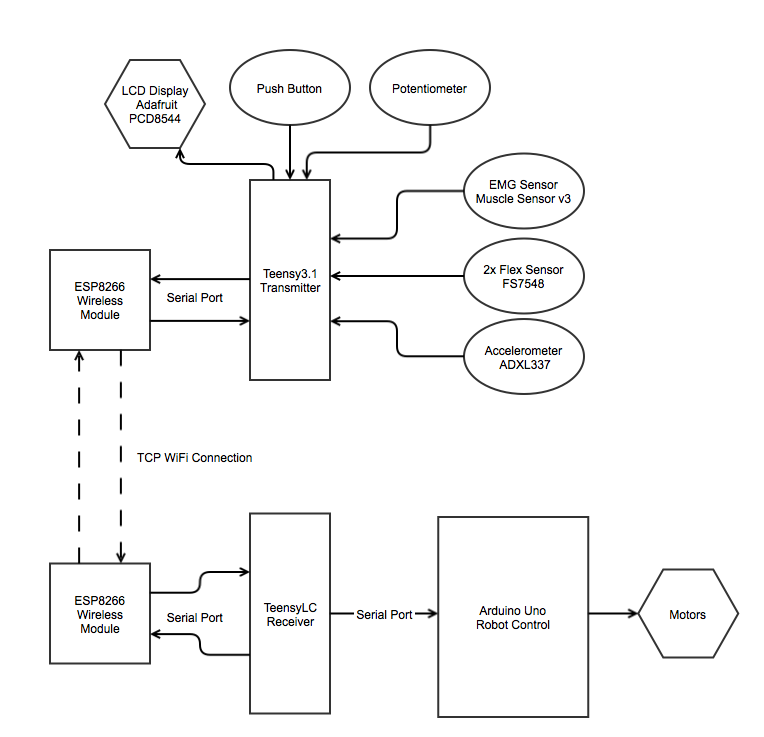
\includegraphics[width=0.8\textwidth]{blkdgrm.png}
  \caption{Block diagram}
\end{figure}

  Below is a brief description of the purpose of each microcontroller, and pseudocode of the software running on each.

  \textbf{Transmitter TeensyLC:} Configure WiFi AP, collect sensor data, transmit commands
  
 {\setstretch{1.0}
  Setup routine:
  \begin{itemize}
    \item Initialize inputs and Adafruit display
    \item Start serial communications
    \item Attach interrupt to push button handler function
    \item Configure ESP8266 as access point
  \end{itemize}
  Main loop:
  \begin{itemize}
  \item Check which sensor is activated and in which way
  \item Prints values to LCD screen
  \item Send a forward, backward, left, right, or stop command in response to glove controller sensors
  \item Send a speed command in response to EMG or potentiometer readings
  \end{itemize}
}

 \textbf{Receiver TeensyLC:} Connect to WiFi AP, translate and pass on commands

 {\setstretch{1.0}
  Setup routine:
  \begin{itemize}
  \item ESP connection and configuration
  \item Start serial communications
  \end{itemize}
  Main loop:
  \begin{itemize}
  \item Detect which direction and speed is being sent by the transmitter
  \item Communicate with the Arduino on the robot (wired)
  \end{itemize}
}

\textbf{Robot Control – Arduino Uno:} Execute robot commands

{\setstretch{1.0}
  Setup routine:
  \begin{itemize}
  \item Start serial communications
  \end{itemize}
  Main loop:
  \begin{itemize}
  \item Position control code from previous labs
  \item Call different direction and speed functions based on what command is received
  \end{itemize}
}

The code is several pages long, so we have created a zip folder containing the final code, which can be found in the references. The code for the transmitter/sensor input TeensyLC is located in ECEN\_TX. This microcontroller maintains configuration of the wireless module, reads sensor input, computes commands for the robot, and sends these to the wireless transmitter module.

The code for the receiver TeensyLC is located in ECEN\_RX. This microcontroller connects to the wireless receiver module, reads commands from it, and passes these commands to the Arduino.

The code for the robot control Arduino Uno is located in Robocode. This microcontroller reads commands from the wireless receiver module and translates them into actions (in this case, driving motors).
  
  \subsubsection{Packaging}

  Several of the input devices, including the accelerometer, the flex sensors, and the EMG were connected to a glove. We also designed a small box that would be attached to the user’s arm. The Teensy, an antenna, batteries, and a screen that displayed the output readings from the glove were placed in the box. The second receiver Teensy was placed on the robot next to all the circuitry from the previous labs. The information from the receiver Teensy was then fed into the Arduino on the robot, which led to motor control.
  
\section{Further Explorations}

If this project were extended and improved upon, a good course of action would be to spend more time on the packaging. For our hand controller we used a garden glove, as that was the best option with the amount of time that was given. However, if there was more time, it would have been a great idea to design and manufacture a glove with plastic coating that made it look like a robot hand. This would have made the project look more complete at the end and would probably result in a more entertaining experience for the user. In addition, more care should have been taken when connecting the EMG muscle sensor up to the batteries. The sensor has both a positive and a negative input voltage, so the user should be very careful when connecting the batteries to ensure that the positive pin receives a positive voltage and the negative pin receives a negative voltage. If the negative pin receives any amount of positive voltage, the sensor will heat up and break.

\section{Conclusion}

Our group successfully demonstrated wireless communication and motor control with the  glove. We were able to implement robot direction control with the flex sensors and accelerometer as well as speed control with both the EMG muscle sensor and the slide potentiometer. The wireless communication proved to be the most difficult part of the project. We initially struggled with establishing the connection between the transmitter and receiver. There was also a lot of code to go through and a few bugs in the program that caused information to be lost between the components. It was more difficult than the last wireless system, but it did have its benefits. WiFi increased our range for the distance the robot could get from the operator while still responding. Using bluetooth could have been an ulterior method that might have been easier to build.

\section{References}

[1]. Teensy Arduino IDE Extension: \url{https://www.pjrc.com/teensy/td_download.html}

[2]. Teensy Reference: \url{https://www.pjrc.com/teensy/}

[3]. TeensyLC Product Page: \url{https://www.pjrc.com/teensy/teensyLC.html}

[4]. ESP8266 Datasheet: \url{https://nurdspace.nl/images/e/e0/ESP8266_Specifications_English.pdf}

[5]. ESP8266 Reference: \url{https://nurdspace.nl/ESP8266}

[6]. GitHub Software Repository: \url{http://github.com/Dacilndak/2270-g121}

[7]. GitHub Software Archive: \url{https://github.com/Dacilndak/2270-g121/archive/master.zip}

\end{document}
